\documentclass[11pt,a4paper]{article}

\usepackage[spanish,es-noshorthands]{babel}
\usepackage[T1]{fontenc}
\usepackage[utf8]{inputenc}
\usepackage{lmodern}
\usepackage[a4paper,margin=2.35cm]{geometry}
\usepackage{amsmath}
\usepackage{amssymb}
\usepackage{booktabs}
\usepackage{array}
\usepackage{tabularx}
\usepackage{graphicx}
\usepackage{float}
\usepackage{caption}
\usepackage{enumitem}
\usepackage{xcolor}
\usepackage{hyperref}
\usepackage{xurl}
\usepackage{natbib}

\hypersetup{
    colorlinks=true,
    linkcolor=blue!60!black,
    citecolor=blue!60!black,
    urlcolor=blue!60!black,
    pdftitle={Guia didactica actualizada del proyecto TD3 para protesis mioelectrica},
    pdfauthor={Proyecto EMG Prosthesis TD3}
}

\newcolumntype{L}[1]{>{\raggedright\arraybackslash}p{#1}}
\newcolumntype{Y}{>{\raggedright\arraybackslash}X}

\title{\textbf{Guia Didactica Actualizada del Proyecto TD3 para una Protesis Mioelectrica}\\
\large Terminos, parametros, formulas y estado final con politica residual}
\author{Proyecto \texttt{EMG\_Prosthesis\_TD3}}
\date{26 de marzo de 2026}

\begin{document}
\maketitle

\begin{abstract}
Esta guia didactica actualiza la ficha conceptual del proyecto hasta su estado final. Explica, con un lenguaje mas pedagogico que el reporte tecnico, que problema resuelve el sistema, que significa cada termino importante, que formulas dominan el comportamiento del agente, que bug cambio la lectura de muchas corridas, como se interpreta el benchmark \texttt{Agent7250} y por que la politica residual \texttt{Agent1850} con \(\alpha_{\mathrm{res}} = 0.20\) se toma como mejor punto final actual. Tambien resume scripts, parametros, criterios de seleccion y nuevas metricas de diagnostico.
\end{abstract}

\tableofcontents
\newpage

\section{Para que sirve esta guia}

Esta guia intenta responder preguntas practicas:
\begin{itemize}[leftmargin=1.5em]
\item Que hace el proyecto exactamente.
\item Que significa cada bloque tecnico importante.
\item Por que se usa TD3.
\item Que se corrige con la reward actual.
\item Que fue el bug del simulador.
\item Que es una politica residual.
\item Que significa alpha\_res.
\item Cual es hoy el mejor agente y por que.
\end{itemize}

\section{Que problema resuelve el proyecto}

El proyecto quiere controlar una protesis robotica de mano a partir de senales EMG. La salida deseada no es un gesto discreto, sino una respuesta continua: cuanto abrir o cerrar cada parte de la protesis en funcion de la actividad muscular del usuario. Esta idea esta alineada con el control mioelectrico moderno \citep{chen2023review} y con el planteamiento base del proyecto \citep{fuertes2026continuous}.

En forma corta:
\[
\text{EMG} \rightarrow \text{estado} \rightarrow \text{actor TD3} \rightarrow \text{accion} \rightarrow \text{simulador} \rightarrow \text{reward}.
\]

\section{Glosario esencial}

\subsection*{EMG}
Actividad electrica muscular. En el proyecto sirve como proxy de la intencion motora.

\subsection*{Features EMG}
Transformaciones numericas de la EMG cruda. Aqui se usan 5 features por cada uno de 8 canales, para un total de 40 dimensiones.

\subsection*{Estado}
Vector que ve el agente en cada paso. En la formulacion valida actual es \texttt{markov52}.

\subsection*{Actor}
Red que produce la accion.

\subsection*{Criticos}
Redes que estiman que tan buena es una accion en un estado. TD3 usa dos criticos \citep{fujimoto2018td3}.

\subsection*{Replay buffer}
Memoria de experiencias pasadas usada para entrenar de forma mas estable.

\subsection*{PWM}
Magnitud de mando aplicada a los motores. En este proyecto la accion del actor termina convertida a niveles efectivos de PWM.

\subsection*{Tracking MSE}
Error cuadratico medio entre referencia y salida de la protesis. Es la metrica central del proyecto.

\subsection*{Tracking MAE}
Error absoluto medio. Es mas interpretable, pero penaliza menos los errores grandes.

\subsection*{ActionL2}
Magnitud media de la accion. Se interpreta como esfuerzo de control.

\subsection*{Saturation fraction}
Fraccion del tiempo en que la accion efectiva queda cerca del borde del actuador.

\subsection*{DeltaActionL2}
Mide cuanto cambia la accion de un paso al siguiente. Es un indicador de brusquedad.

\subsection*{Checkpoint}
Agente guardado durante entrenamiento. El mejor agente no tiene por que ser el ultimo.

\subsection*{Auditoria de checkpoints}
Proceso de evaluar varios checkpoints con simulaciones cortas y largas para seleccionar el mejor por metricas reales, no por reward final de entrenamiento.

\subsection*{ConditionA y ConditionB}
Reglas de aceptacion frente al benchmark \texttt{Agent7250}. \texttt{ConditionA} exige mejora estricta. \texttt{ConditionB} permite perder muy poco tracking a cambio de bajar bastante saturacion y esfuerzo.

\subsection*{Politica base}
En la fase final es \texttt{Agent7250}. Sobre ella se construye la correccion residual.

\subsection*{Politica residual}
Politica que no reemplaza totalmente a la base, sino que aprende una correccion pequena.

\subsection*{alpha\_res}
Escala que multiplica la correccion residual. Controla cuanto puede apartarse el agente final de la accion base.

\section{Por que se usa TD3}

TD3 es apropiado porque este proyecto es de accion continua, no de clasificacion discreta. Su logica central es:
\begin{itemize}[leftmargin=1.5em]
\item dos criticos para reducir sobreestimacion;
\item actualizacion mas lenta del actor;
\item suavizado de la politica objetivo.
\end{itemize}

Eso lo vuelve una buena opcion para control continuo con ruido y estados complejos \citep{fujimoto2018td3,mathworks_td3_agent,mathworks_td3_options}.

\section{Estado y accion del proyecto}

\subsection{Observacion markov52}

La observacion valida actual se puede resumir como:
\[
s_t=
\begin{bmatrix}
\phi_t \\
\mathrm{enc}_t \\
\Delta \mathrm{enc}_t \\
\tilde{a}_{t-1}
\end{bmatrix}
\in \mathbb{R}^{52},
\]
donde:
\begin{itemize}[leftmargin=1.5em]
\item \(\phi_t \in \mathbb{R}^{40}\): features EMG;
\item \(\mathrm{enc}_t \in \mathbb{R}^{4}\): encoders normalizados;
\item \(\Delta \mathrm{enc}_t \in \mathbb{R}^{4}\): cambio de encoder;
\item \(\tilde{a}_{t-1} \in \mathbb{R}^{4}\): accion efectiva previa.
\end{itemize}

\subsection{Accion del actor}

El actor produce:
\[
a_t \in [-1,1]^4.
\]

Pero eso no significa que la protesis reciba exactamente ese valor continuo. Antes de actuar, la accion se remapea y se cuantiza a niveles efectivos. Esa es una idea crucial del repo: una politica buena no se juzga solo por su accion cruda, sino por la accion efectiva que termina recibiendo el actuador.

\section{La reward actual y por que esta bien planteada}

La reward vigente es:
\[
r_t = -\frac{1}{4}\sum_{i=1}^{4}\left(
e_{t,i}^{2}
\lambda_a \tilde{a}_{t,i}^{2}
\lambda_{\Delta a}\left(\tilde{a}_{t,i}-\tilde{a}_{t-1,i}\right)^2
\right).
\]

Donde:
\begin{itemize}[leftmargin=1.5em]
\item \(e_{t,i}\): error de tracking;
\item \(\lambda_a\): peso del esfuerzo de accion;
\item \(\lambda_{\Delta a}\): peso de la suavidad.
\end{itemize}

La idea pedagogica es:
\begin{itemize}[leftmargin=1.5em]
\item el tracking manda;
\item el esfuerzo se regulariza;
\item la brusquedad tambien se regulariza.
\end{itemize}

Esto es mucho mas interpretable que la reward heredada inicial y evita parte de los problemas clasicos de \emph{reward shaping} mal alineado \citep{deng2025reward,lee2024smoothness}.

\section{El bug del simulador explicado de forma sencilla}

Una parte importante del proyecto consistio en descubrir que el simulador no estaba moviendo de verdad a la protesis en ciertas corridas antiguas. En otras palabras:
\begin{itemize}[leftmargin=1.5em]
\item el agente ``entrenaba'',
\item la reward cambiaba,
\item pero la planta no reaccionaba correctamente.
\end{itemize}

Eso fue grave porque invalidaba comparaciones numericas. Despues del fix, el proyecto entro en su fase valida. Esta es la razon por la que el benchmark serio no se toma de las corridas antiguas, sino de las corridas post-fix.

\section{Linea valida antes de la fase residual}

\begin{table}[H]
\centering
\caption{Linea post-fix principal antes de la mejora residual}
\begin{tabular}{lrrrrr}
\toprule
Etapa & trackingMSE & trackingMAE & actionL2 & saturationFraction & deltaActionL2 \\
\midrule
Baseline post-fix de 2000 episodios & 0.052805 & 0.179093 & 0.674957 & 0.474999 & 0.633264 \\
\texttt{Agent7250} en 8000 episodios & 0.043045 & 0.160336 & 0.596444 & 0.392086 & 0.321385 \\
\texttt{Agent11900} en 12000 episodios & 0.045189 & 0.164639 & 0.649868 & 0.511786 & 0.305285 \\
\bottomrule
\end{tabular}
\end{table}

Leccion didactica:
\begin{itemize}[leftmargin=1.5em]
\item mas episodios no garantizan una politica mejor;
\item el mejor checkpoint debe elegirse por auditoria;
\item un mejor reward final de entrenamiento no basta para declarar victoria.
\end{itemize}

\section{Que se intento despues de Agent7250}

Despues del benchmark \texttt{Agent7250} se probaron varias ideas porque el tracking ya era bueno, pero el control seguia siendo algo agresivo.

\subsection{Baja exploracion}
Se bajo el ruido de exploracion buscando una politica mas suave. Mejoro esfuerzo y saturacion, pero el tracking cayo demasiado.

\subsection{Threshold-aware exploration}
Se exploto el hecho de que el actuador tiene una discontinuidad real entre umbral y primer bin efectivo. Sirvio para entender mejor el repo, pero no produjo un agente nuevo mejor.

\subsection{Reward con saturacion}
Busco penalizar explicitamente cercania al borde. Resultado: politicas demasiado timidas.

\subsection{Warm-start offline}
Introdujo un prior mas suave desde datos sinteticos. Resultado: politicas demasiado conservadoras.

\subsection{Interfaz de accion alineada}
Intento hacer coincidir mejor la salida continua del actor con los niveles realmente utiles del actuador. Resultado: politicas demasiado agresivas.

\subsection{Residual TD3}
No intento reemplazar la politica base, sino corregirla. Esta fue la unica linea que produjo una mejora real.

\section{Que es una politica residual}

La politica residual final del proyecto se escribe como:
\[
a(s)=\mathrm{clip}\Big(a_{\mathrm{base}}(s)+\alpha_{\mathrm{res}}\,a_{\mathrm{res}}(s,a_{\mathrm{base}}),-1,1\Big).
\]

Interpretacion sencilla:
\begin{itemize}[leftmargin=1.5em]
\item \(a_{\mathrm{base}}\): lo que haria \texttt{Agent7250};
\item \(a_{\mathrm{res}}\): una correccion aprendida;
\item \(\alpha_{\mathrm{res}}\): cuanto poder se le da a esa correccion.
\end{itemize}

Si \(\alpha_{\mathrm{res}}\) es pequeno, la residual apenas corrige. Si es grande, la residual puede separarse mucho de la base. El proyecto encontro que el mejor equilibrio estaba en \(\alpha_{\mathrm{res}} = 0.20\).

\section{Parametros importantes del estado final}

\begin{table}[H]
\centering
\caption{Parametros clave del estado final del proyecto}
\begin{tabularx}{\linewidth}{L{5.0cm}L{2.7cm}Y}
\toprule
Parametro & Valor & Que significa \\
\midrule
\texttt{observationVariant} & \texttt{markov52} & Estado valido actual. \\
\texttt{rewardType} & \texttt{trackingMseActionRateReward} & Reward base del proyecto. \\
\texttt{agent\_id} & \texttt{td3\_residual7250} & Familia final del agente. \\
\texttt{td3.useRecurrent} & \texttt{false} & La linea final es feedforward, no LSTM. \\
\texttt{td3Residual.baseCheckpointPath} & \texttt{Agent7250} & Politica base congelada. \\
\texttt{td3Residual.residualScale} & \texttt{0.20} & Mejor escala residual encontrada. \\
\texttt{td3Residual.hiddenUnits} & \texttt{32} & Anchura de la rama residual. \\
\texttt{explorationStd} & \texttt{0.02} & Ruido de exploracion residual. \\
\texttt{explorationStdMin} & \texttt{0.002} & Piso del ruido residual. \\
\texttt{explorationStdDecayRate} & \texttt{1e-4} & Decaimiento del ruido. \\
\texttt{rewardActionWeight} & \texttt{0.01} & Penalizacion de magnitud de accion. \\
\texttt{rewardDeltaActionWeight} & \texttt{0.05} & Penalizacion de cambio de accion. \\
\texttt{trainingEpisodes} & \texttt{2000} & Longitud de la corrida residual principal. \\
\texttt{trainingSaveAgentEvery} & \texttt{50} & Frecuencia de checkpoints. \\
\bottomrule
\end{tabularx}
\end{table}

\section{Metricas y diagnosticos nuevos de la fase residual}

La fase residual anadio diagnosticos utiles:

\begin{itemize}[leftmargin=1.5em]
\item \texttt{baseActionLog}: que habria hecho la politica base;
\item \texttt{residualActionLog}: cuanto corrige la residual;
\item \texttt{ResidualActionL2Mean}: magnitud media de la correccion;
\item \texttt{BaseToFinalActionDeltaMean}: cuanto se separa la accion final de la base;
\item \texttt{SignOverrideFractionMean}: cuantas veces la residual cambia el signo de la accion base.
\end{itemize}

Estos terminos ayudan a responder una pregunta importante: la residual esta corrigiendo con moderacion o esta intentando reemplazar por completo a la politica base.

\section{Barridos de alpha\_res}

Hubo dos barridos:
\begin{itemize}[leftmargin=1.5em]
\item sweep corto: \(\{0.10, 0.20, 0.30\}\),
\item refinamiento fino: \(\{0.18, 0.20, 0.22, 0.25\}\).
\end{itemize}

Resultado didactico:
\begin{itemize}[leftmargin=1.5em]
\item valores bajos no corrigieron bien;
\item valores altos compraron mejora local de tracking con demasiado borde o esfuerzo;
\item \(\alpha_{\mathrm{res}} = 0.20\) fue el punto util.
\end{itemize}

\begin{figure}[H]
\centering
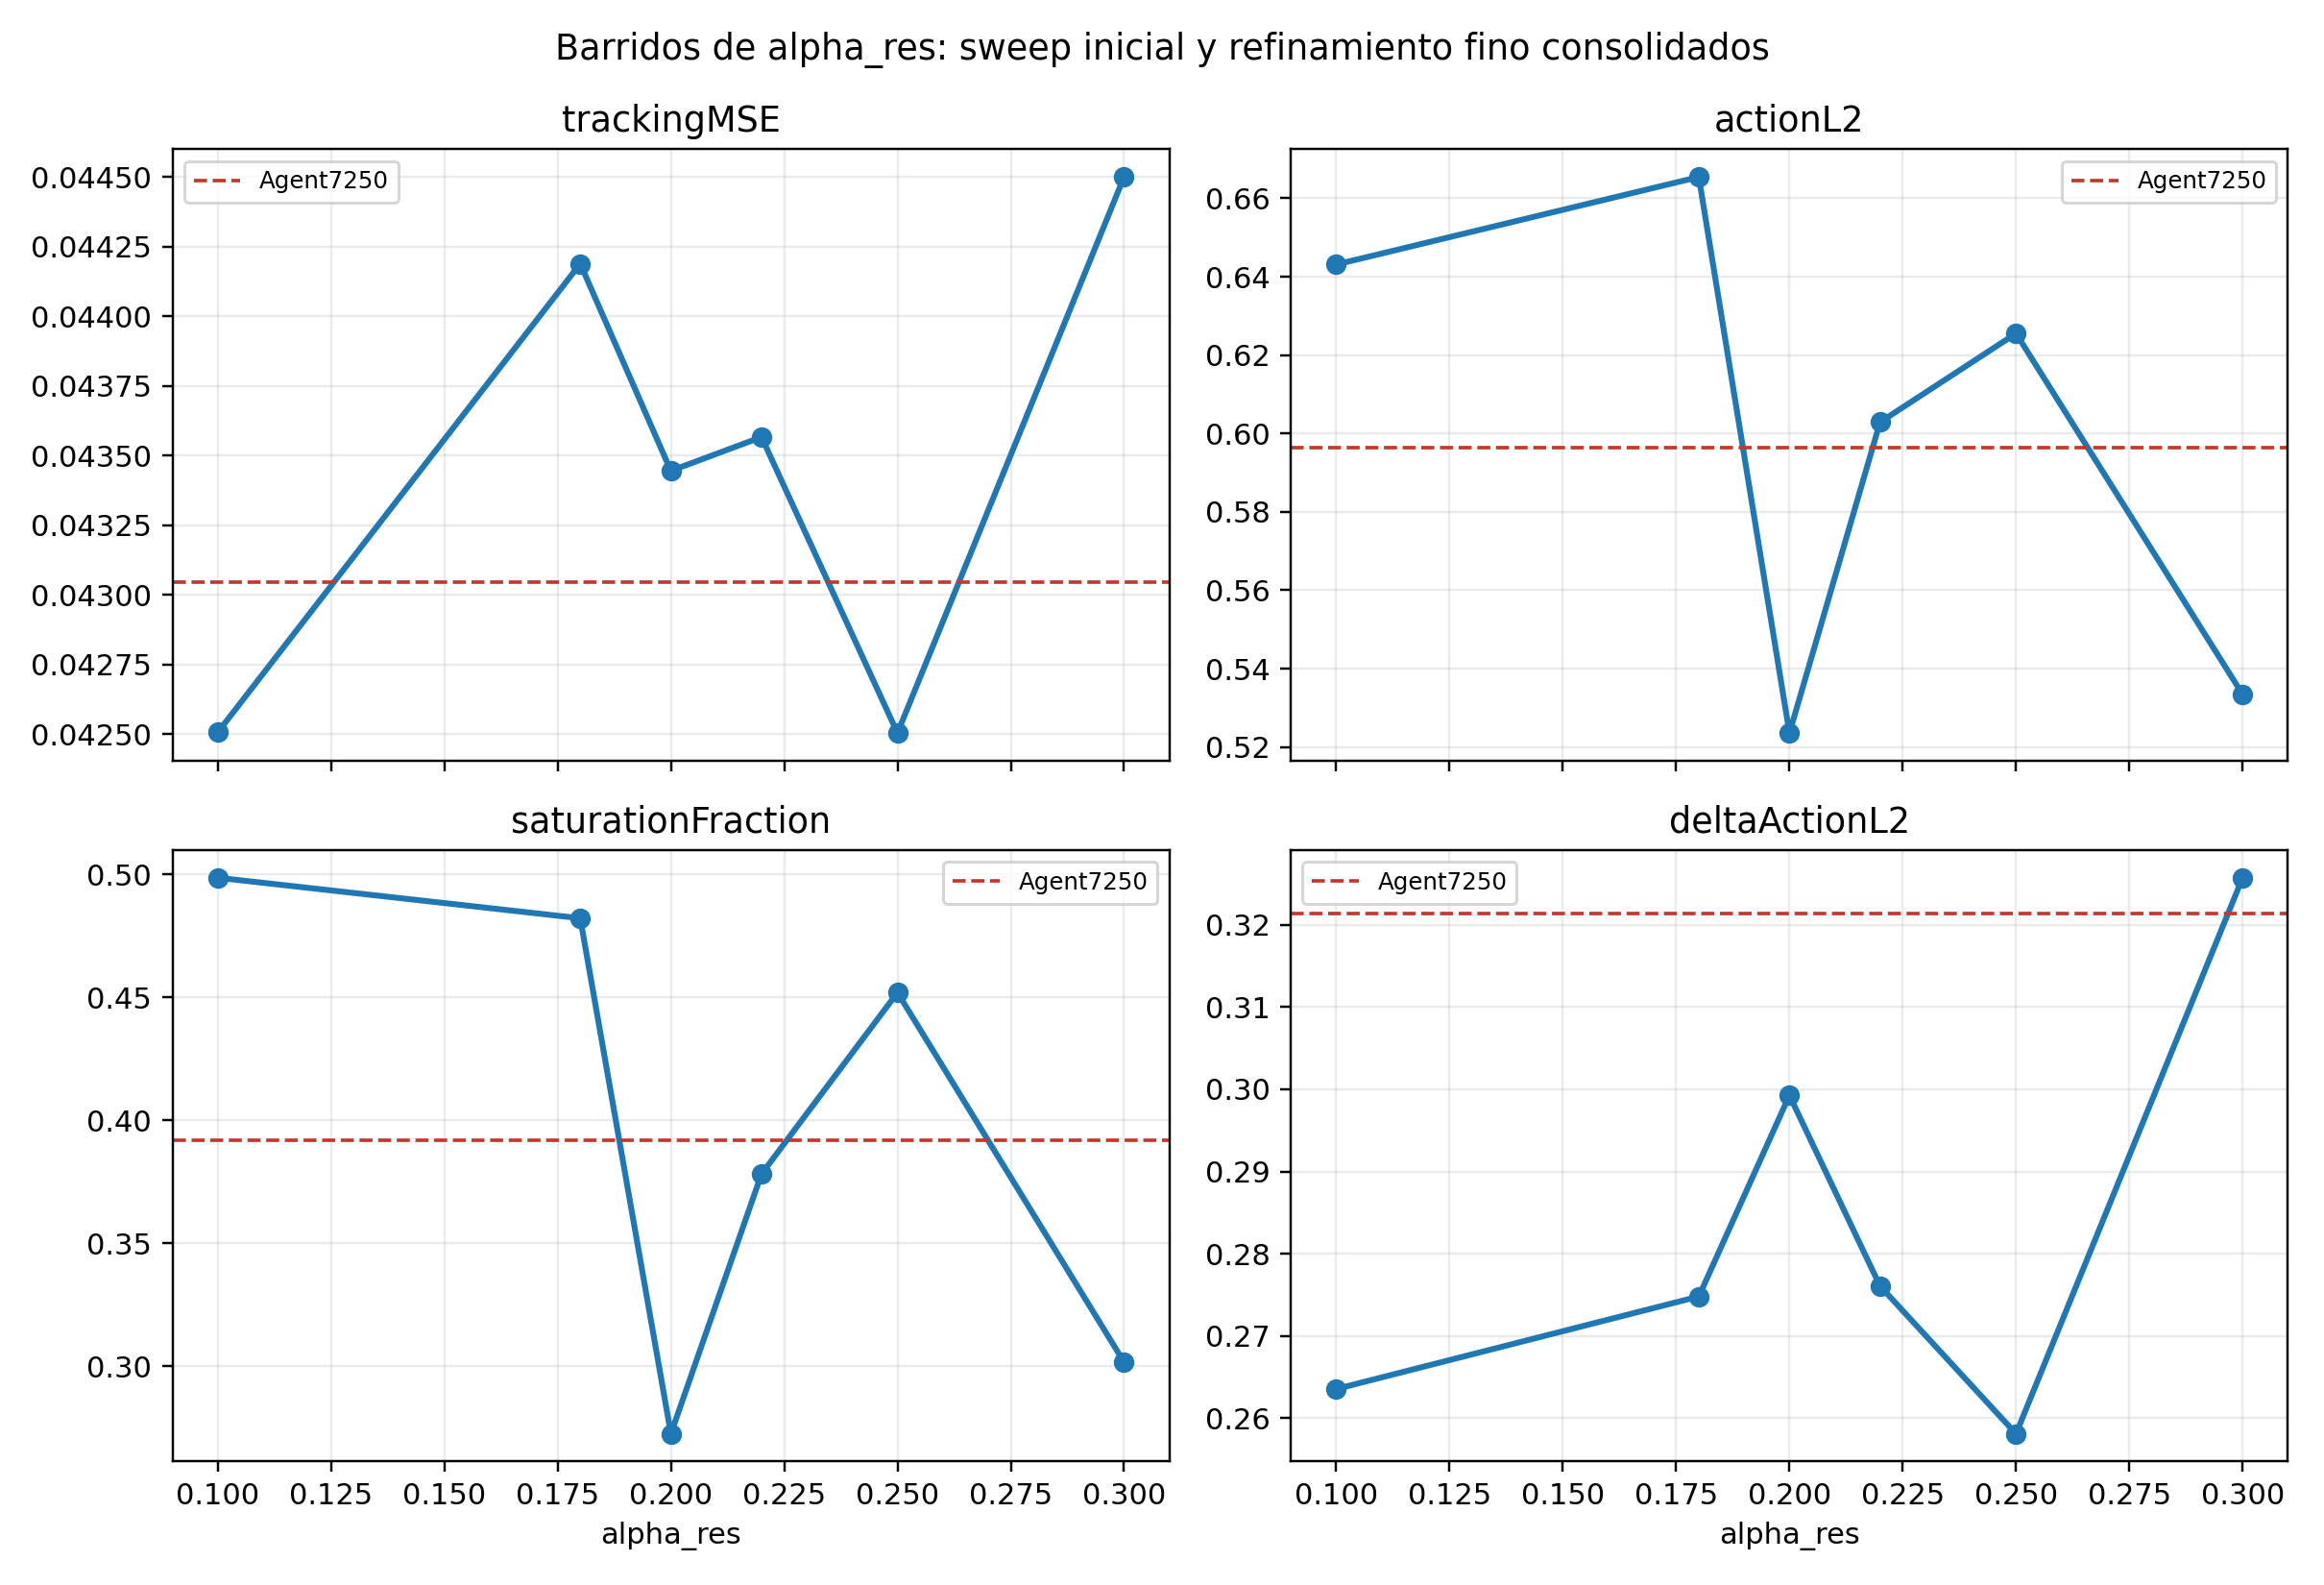
\includegraphics[width=0.95\linewidth]{figures/residual_alpha_sweep_metrics_20260326.png}
\caption{Barridos de alpha\_res respecto al benchmark.}
\end{figure}

\begin{figure}[H]
\centering
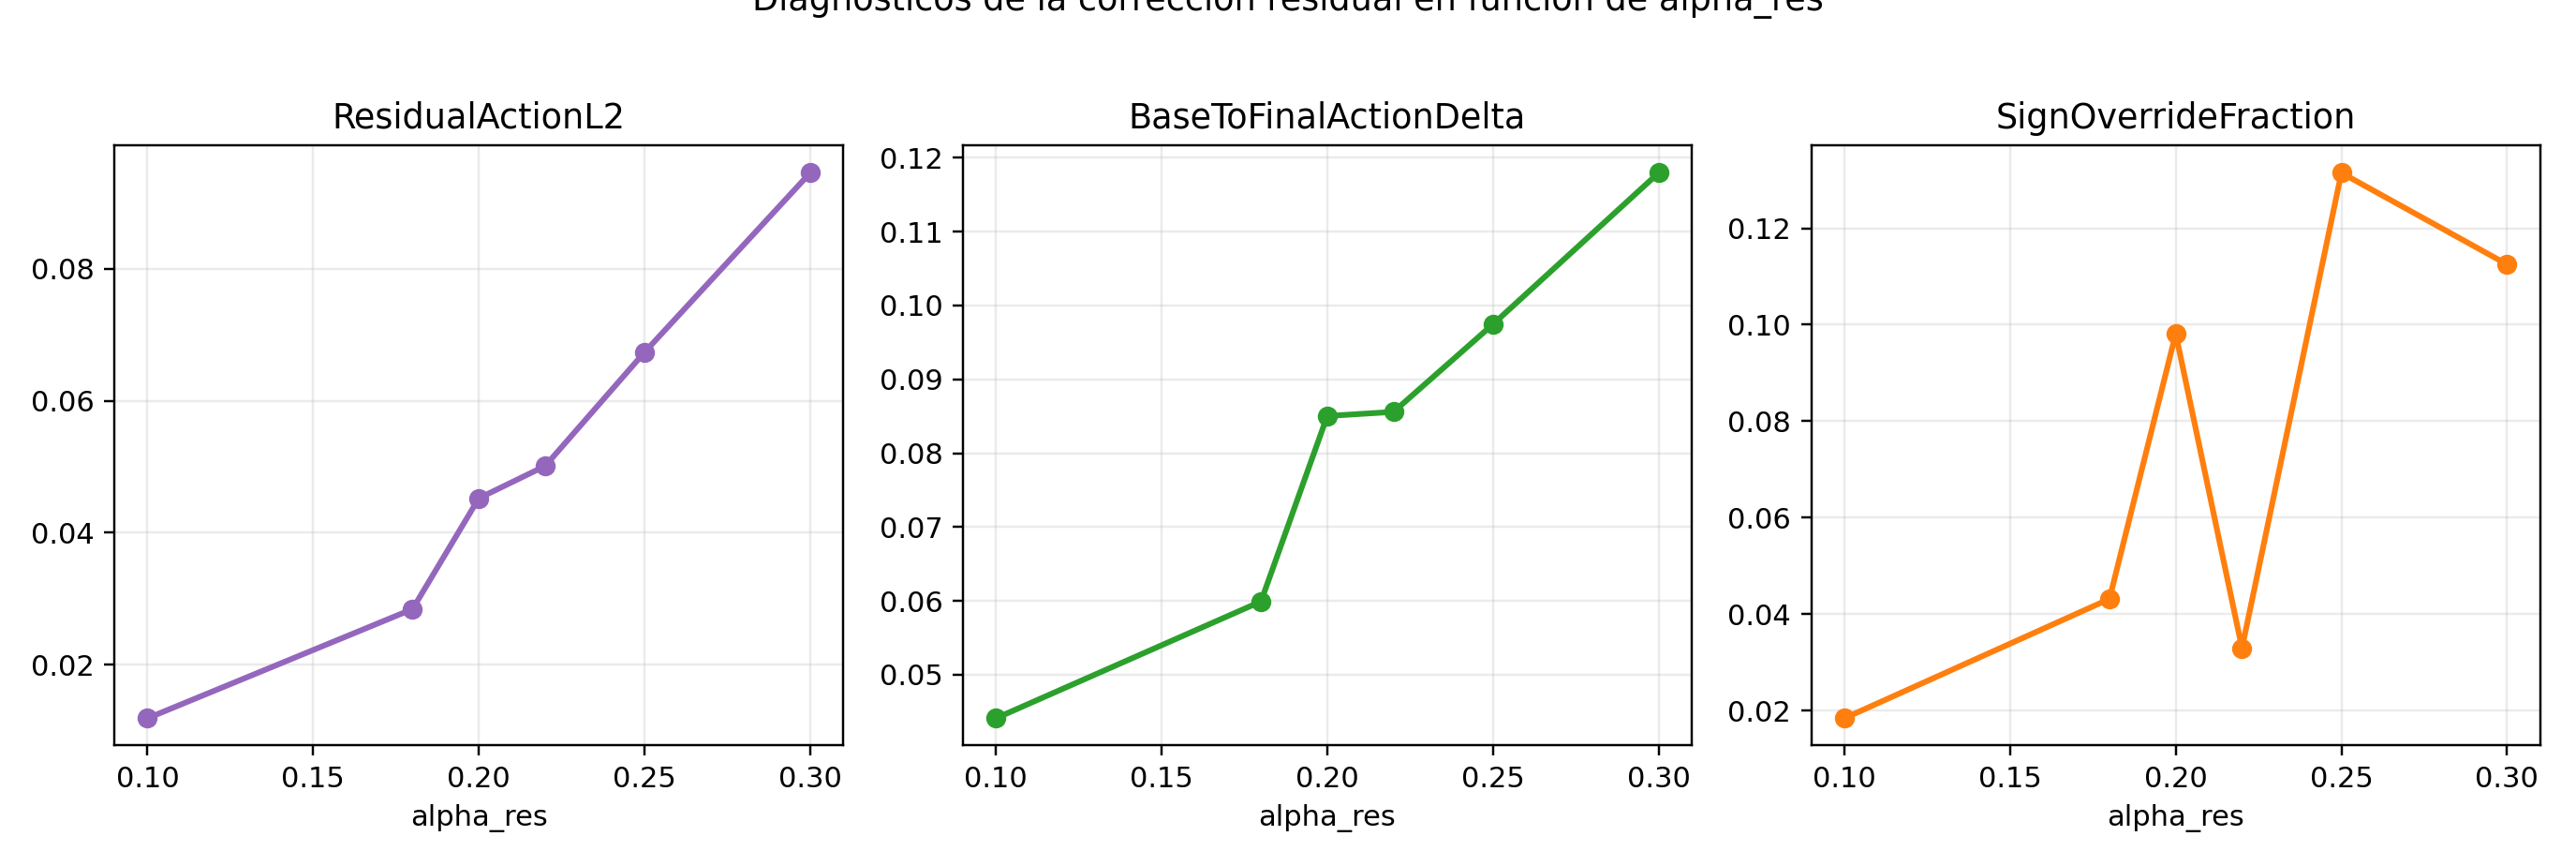
\includegraphics[width=0.95\linewidth]{figures/residual_alpha_diagnostics_20260326.png}
\caption{Diagnosticos de la correccion residual. La zona de alpha=0.20 mantiene una correccion util y moderada.}
\end{figure}

\section{Agente final del proyecto}

El mejor candidato final actual es:
\begin{itemize}[leftmargin=1.5em]
\item base congelada: \texttt{Agent7250},
\item mejora final: residual \texttt{Agent1850} con \(\alpha_{\mathrm{res}}=0.20\).
\end{itemize}

\begin{table}[H]
\centering
\caption{Comparacion final entre benchmark y mejor residual}
\begin{tabular}{lrr}
\toprule
Metrica & \texttt{Agent7250} & Residual \texttt{Agent1850} \\
\midrule
\texttt{trackingMSE} & 0.043045 & 0.043445 \\
\texttt{trackingMAE} & 0.160336 & 0.163542 \\
\texttt{actionL2} & 0.596444 & 0.523597 \\
\texttt{saturationFraction} & 0.392086 & 0.272637 \\
\texttt{deltaActionL2} & 0.321385 & 0.299262 \\
\bottomrule
\end{tabular}
\end{table}

Interpretacion corta:
\begin{itemize}[leftmargin=1.5em]
\item el tracking casi no empeora;
\item la saturacion baja mucho;
\item el esfuerzo de control baja;
\item por eso el resultado final entra en \texttt{ConditionB}.
\end{itemize}

\begin{figure}[H]
\centering
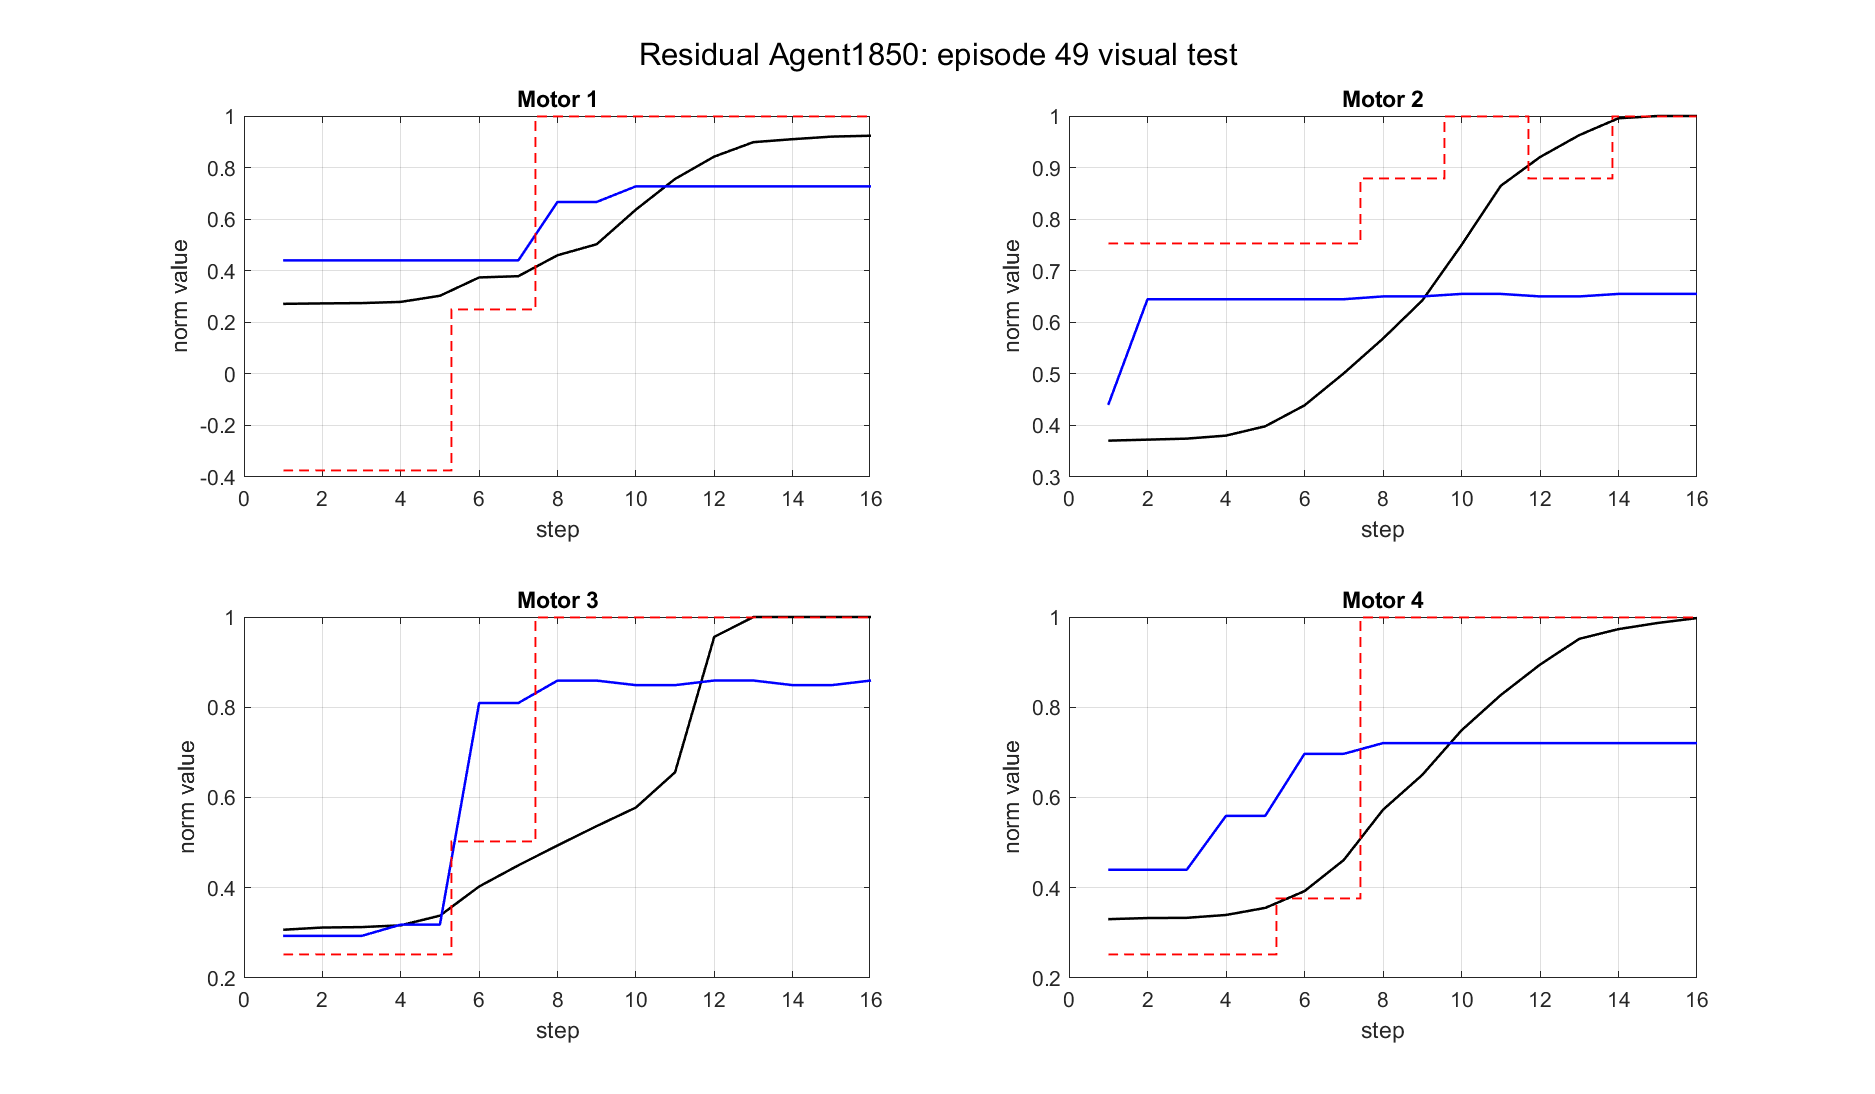
\includegraphics[width=0.92\linewidth]{figures/residual_agent1850_episode49_20260326.png}
\caption{Ejemplo del test visual del residual \texttt{Agent1850}.}
\end{figure}

\section{Scripts y flujos importantes}

\begin{table}[H]
\centering
\caption{Scripts importantes del estado final}
\begin{tabularx}{\linewidth}{L{5.5cm}Y}
\toprule
Script & Para que sirve \\
\midrule
\texttt{trainInterface('td3','','')} & Flujo general de entrenamiento y test del baseline TD3. \\
\texttt{runCheckpointAudit(...)} & Audita checkpoints con fase rapida y fase completa. \\
\texttt{runCheckpointTest(...)} & Ejecuta test visual y metricas agregadas. \\
\texttt{run\_agent7250\_residual\_policy\_pilot} & Lanza el piloto residual principal. \\
\texttt{run\_agent7250\_residual\_continuation} & Continua desde el mejor residual. \\
\texttt{run\_agent7250\_residual\_alpha\_sweep} & Ejecuta el barrido corto de alpha. \\
\texttt{run\_agent7250\_residual\_alpha\_refinement\_sweep} & Ejecuta el refinamiento fino de alpha. \\
\bottomrule
\end{tabularx}
\end{table}

\section{Idea final que debe quedar clara}

La leccion didactica mas importante del proyecto es esta:

\begin{quote}
la mejora final no vino de volver a cambiar reward, ni de meter mas episodios sin criterio, ni de reconstruir todo desde cero; vino de partir de una politica base fuerte y aprender una correccion residual pequena, bien medida y auditada.
\end{quote}

Ese es el punto final conceptual y operativo del proyecto actual.

\bibliographystyle{unsrt}
\bibliography{references}

\end{document}
